\chapter{System Requirements, Design, and Implementation}



\section{Requirements Specification}
The System Requirements Specification (SRS) provides a comprehensive and detailed description of the Place Names Information System (PNIS). It serves as a blueprint for recording data, describing functionalities, and setting performance and design constraints. This SRS ensures a clear understanding of the system's objectives, requirements, and users' expectations, facilitating a systematic approach to development. This document also helps maintain consistency and ensures that the application meets user needs and thesis goals.

\subsection{Features}
The PNIS connects with a database to store and retrieve information about locations, administrative areas, and other related aspects such as historical data, alternative names, geographical attributes, and user-generated information.
Administrative details provide the foundation for understanding the geographical and administrative context of a location. The system enhances searchability and discovery by incorporating various names a location may have, thus improving data accessibility. Geographical features offer a deeper understanding of a location’s physical characteristics, while historical data enrich locations with stories and events that have occurred over time.

\subsection{Functional Requirements}

\subsubsection{User Management}
Users will be able to register, login, and logout. The application will authenticate users based on securely stored usernames and passwords and will implement mechanisms to reset forgotten passwords. An admin user type will exist with elevated privileges.

\subsubsection{Location Management}
Users will be able to search for locations based on various criteria such as name and postal code. The application will display details of a location including its description, founding year (if available), and alternative names. Authorized users will be allowed to add new locations with descriptions and basic details.

\subsubsection{Content Management}
Users will be able to create and submit posts related to locations. The system will implement a workflow for administrators to approve or reject posts. Users will be able to view posts associated with specific locations and add comments to existing posts.

\subsubsection{Administrative Functions}
Admin users will be able to manage user accounts, update administrative details, and potentially manage other aspects of the data.

\subsection{Non-Functional Requirements}

\subsubsection{Performance}
The system shall be capable of handling large volumes of data efficiently. Data retrieval and query processing shall be optimized for responsiveness, and algorithms for data acquisition shall be designed for scalability and performance.

\subsubsection{Security}
Access to the system shall be role-based with different levels of permissions for users. Data stored within the system shall be encrypted to ensure confidentiality and integrity. Measures shall be in place to prevent unauthorized access and data breaches.

\subsection{Data Model Diagram and Description}
Below is the model schematic diagram that provides overall model functionality features:

\begin{figure}[H]
    \centering
    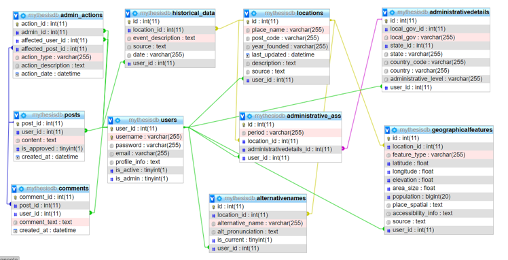
\includegraphics[width=1\linewidth]{model_schema.png}
    \caption{Data Model (Database Schematic) Diagram}
    \label{fig:enter-label}
\end{figure}

\subsubsection{Diagram Descriptions}
The \textit{administrativedetails} table stores administrative area information such as country, state, and local government. The \textit{administrative\_ass} table stores associations between administrative areas and specific identifiers (location\_id) during a specific period. The \textit{admin\_actions} table tracks actions taken by administrators on the system, including affected users or posts. The \textit{alternativenames} table stores alternative names for locations. The \textit{comments} table stores information about comments made on posts, including the content and the user who created it. The \textit{geographicalfeatures} table stores geographical features associated with locations, including type, location data, and descriptions. The \textit{historical\_data} table stores historical data and events related to locations, including event descriptions, sources, and dates. The \textit{locations} table contains information about specific locations, including name, postal code, founding year, and descriptions. The \textit{posts} table stores posts created by users, including content, approval status, and creation time. The \textit{users} table stores information about users, including username, password, email, profile information, and account status.

\section{Design Specification}
The Place Names Information System (PNIS) is designed to record, manage, and analyze data related to place names and their attributes. The system aims to provide a comprehensive platform for users to explore and learn about various locations in Edo-Benin City. Below is a detailed blueprint of the system architecture, illustrating how the requirements were implemented.

\subsection{System Architecture Overview}
The architecture of PNIS is designed to be modular, scalable, and secure, ensuring that it can efficiently handle large volumes of data and provide a robust user experience. The system is divided into several layers, each responsible for specific functionalities:

\subsubsection{Presentation Layer}
Developed using HTML, CSS, JavaScript, and AJAX to create a responsive and user-friendly interface. The front-end application will interact with the back-end services through RESTful APIs.

\subsubsection{Application Layer}
Uses PHP for server-side processing, handling requests from the front end and interacting with the database. The server will manage user sessions, authenticate users, and process CRUD operations.

Facilitates communication between the front-end application and the database. The API will support operations for user management, location management, and content management.

\subsubsection{Data Layer}
A MySQL relational database designed to store and manage all data related to locations, administrative details, user information, and more. The database schema is normalized to reduce redundancy and improve data integrity.

Handles the integration of data from various sources, including public APIs (e.g., OpenStreetMap), manual data entry, and bulk uploads. This module ensures that data is accurately imported and mapped to the database schema.

\subsubsection{Security Layer}
Implements role-based access control (RBAC) to ensure that only authorized users can access specific features. User passwords are securely stored using hashing algorithms.

\subsection{Implementation Details of Requirements}

\subsubsection{User Management}
The system provides a robust user management framework that allows users to register, log in, and manage their accounts. During registration, users can create an account by providing a username, email, and password. The system validates these inputs and securely stores the credentials. Upon successful registration, users gain access to their accounts through the login feature. Additionally, the system includes mechanisms for password management, enabling users to reset forgotten passwords securely via email verification and token-based authentication. Admin users are equipped with elevated privileges, allowing them to manage user accounts, review content, and perform other administrative tasks efficiently.

\subsubsection{Location Management}
The location management functionality enables users to search for and discover locations using various criteria, such as name, postal code, and alternative names. The search functionality is optimized for quick data retrieval, ensuring users can find relevant information promptly. Detailed information about each location, including its description, founding year, and alternative names, is displayed. Authorized users have the capability to add new locations, complete with relevant details, ensuring the database remains comprehensive and up-to-date.

\subsubsection{Content Management}
The content management system allows users to create and submit posts related to specific locations. These posts can include descriptions, historical data, and personal experiences, enriching the dataset with diverse perspectives. An approval workflow is implemented, whereby administrators review submitted posts and approve or reject them based on predefined criteria. This process ensures that only relevant and accurate content is published. Additionally, users can comment on posts, fostering community interaction and engagement. Comments are moderated to maintain quality and relevance, ensuring the platform remains a valuable resource for all users.

\subsubsection{Administrative Functions}
Administrative functions are designed to provide comprehensive control over the system's data and user interactions. Admin users can manage user accounts, including activating or deactivating accounts and updating user information as needed. Data management capabilities allow administrators to update administrative details, manage locations, and oversee the overall data integrity. This ensures that the system remains accurate, reliable, and useful for all stakeholders.


\section{Implementation of Place Names Information System}
The implementation of the Place Names Information System (PNIS) transforms the design specifications into a functional system. This process encompasses coding various components to ensure they work together seamlessly to meet the specified requirements. The following sections provide a detailed discussion on how the system was implemented.

\subsection{Front-End Development}
The front-end development focused on creating a responsive and user-friendly interface, enabling users to interact with the system efficiently. HTML and CSS were employed for structuring and styling the web pages, ensuring a consistent and visually appealing design. JavaScript and AJAX were used to handle asynchronous requests, enhancing user experience by dynamically updating content without requiring full page reloads.

A key feature of the front end is the search bar, allowing users to search for locations using various criteria such as name, postal code, and alternative names. AJAX calls were utilized to fetch and display real-time search results, ensuring a seamless and interactive user experience.

\subsection{Back-End Development}
The back-end development was implemented using PHP, which handles server-side processing, including user authentication, data processing, and interaction with the database. RESTful APIs were set up to facilitate communication between the front-end application and the database. These APIs manage CRUD (Create, Read, Update, Delete) operations for user management, location management, and content management.

MySQL was chosen as the relational database management system (RDBMS). The database schema was designed to capture relationships between different entities, ensuring data normalization and integrity. SQL queries and stored procedures were developed to efficiently retrieve and manipulate data based on user inputs and actions.

\subsection{Data Acquisition and Integration}
The system integrates with public APIs, such as OpenStreetMap, to fetch location data. Custom APIs were developed to connect with external data sources, ensuring data is retrieved in a structured and consistent format. User-friendly interfaces for manual data entry were also developed, allowing the enrichment of the database with user entries under specified standards.

Bulk upload capabilities were enabled, allowing the import of data files (e.g., CSV, Excel) from trusted sources such as libraries and local post offices. Data mapping techniques were used to align imported data with the database schema, ensuring proper field matching and type conversion.

\subsection{Data Preprocessing and Storage}
To ensure data quality, automated scripts and manual review processes were implemented to identify and merge duplicate records, handle missing values, and correct errors. Techniques such as imputation and normalization were used to maintain data integrity.

Data was normalized to fit the relational database schema, ensuring each piece of data is stored in the appropriate table and field. New features were created from raw data to enhance the database, such as calculating population density from area size and population data. Data from multiple sources was merged, resolving conflicts and discrepancies through predefined rules and priority settings. Schema mapping was employed to align data from different sources with the existing database schema.

\subsection{Security Implementation}
Robust security measures were implemented to protect user data and system integrity. Role-based access control (RBAC) ensures that only authorized users can perform specific actions. PHP's built-in cryptography extension was used for password hashing, securely storing user passwords. Additionally, users are provided with mechanisms to reset forgotten passwords securely through email verification and token-based authentication.

In conclusion, the implementation of the Place Names Information System (PNIS) involved meticulous planning and execution across multiple development stages. From front-end and back-end development to data acquisition, preprocessing, and security implementation, each component was carefully crafted to ensure a comprehensive, reliable, and user-friendly system.